
\begin{figure}[t]
\centering
% First row of images
\subcaptionbox{Raw data\label{fig:data}}
{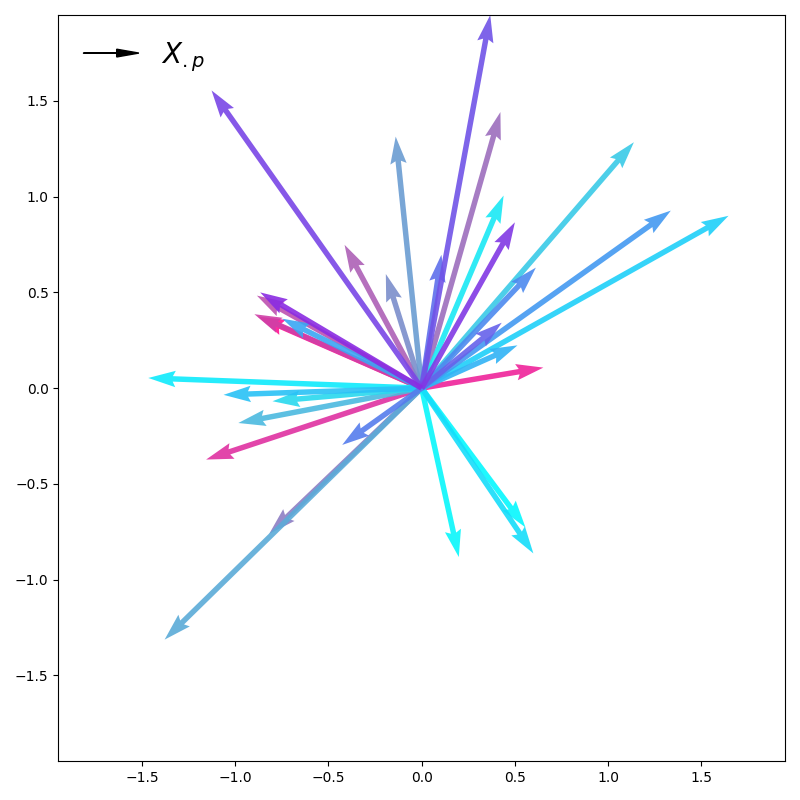
\includegraphics[width = .32\textwidth]{/Users/samsonkoelle/isometry-pursuit/figures/data.png}}
\subcaptionbox{Isometric subset\label{fig:selection}}
{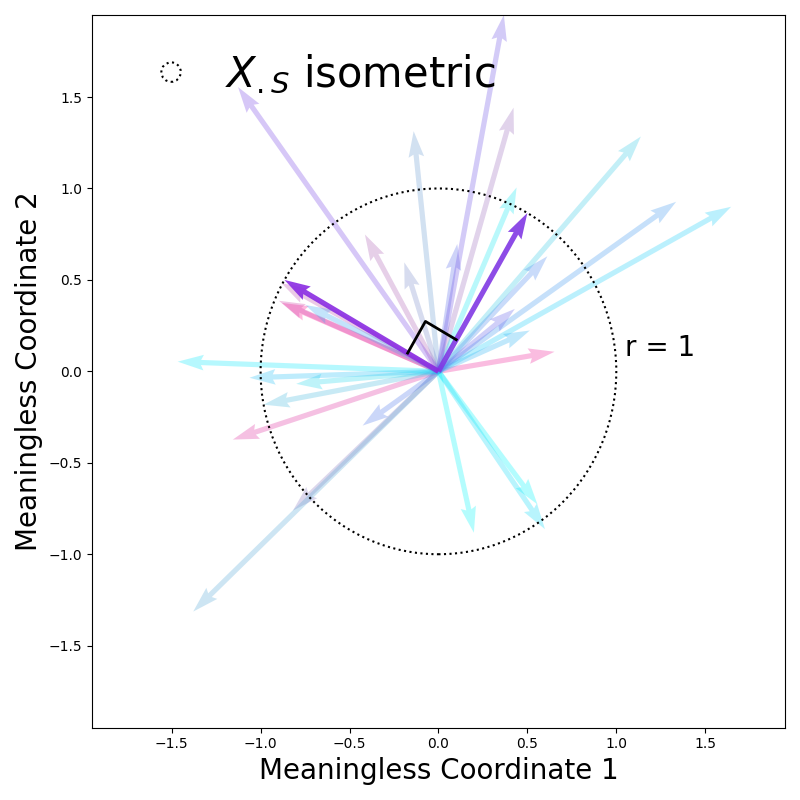
\includegraphics[width = .32\textwidth]{/Users/samsonkoelle/isometry-pursuit/figures/selection.png}}
\subcaptionbox{Normalization step\label{fig:normalization}}
{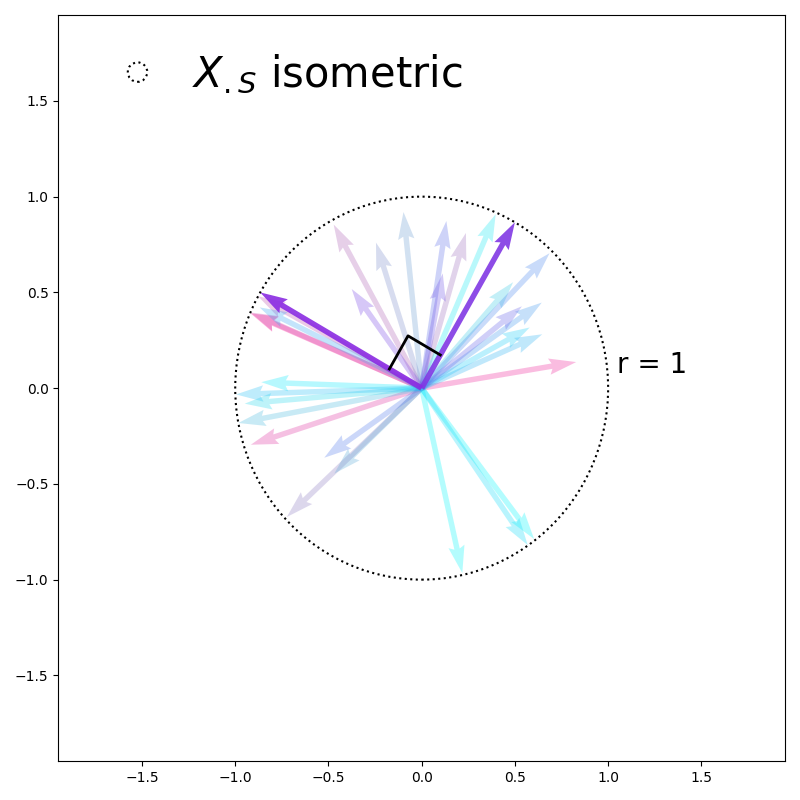
\includegraphics[width = .32\textwidth]{/Users/samsonkoelle/isometry-pursuit/figures/normalization.png}}
\subcaptionbox{Ground truth loss\label{fig:gt_loss}}
{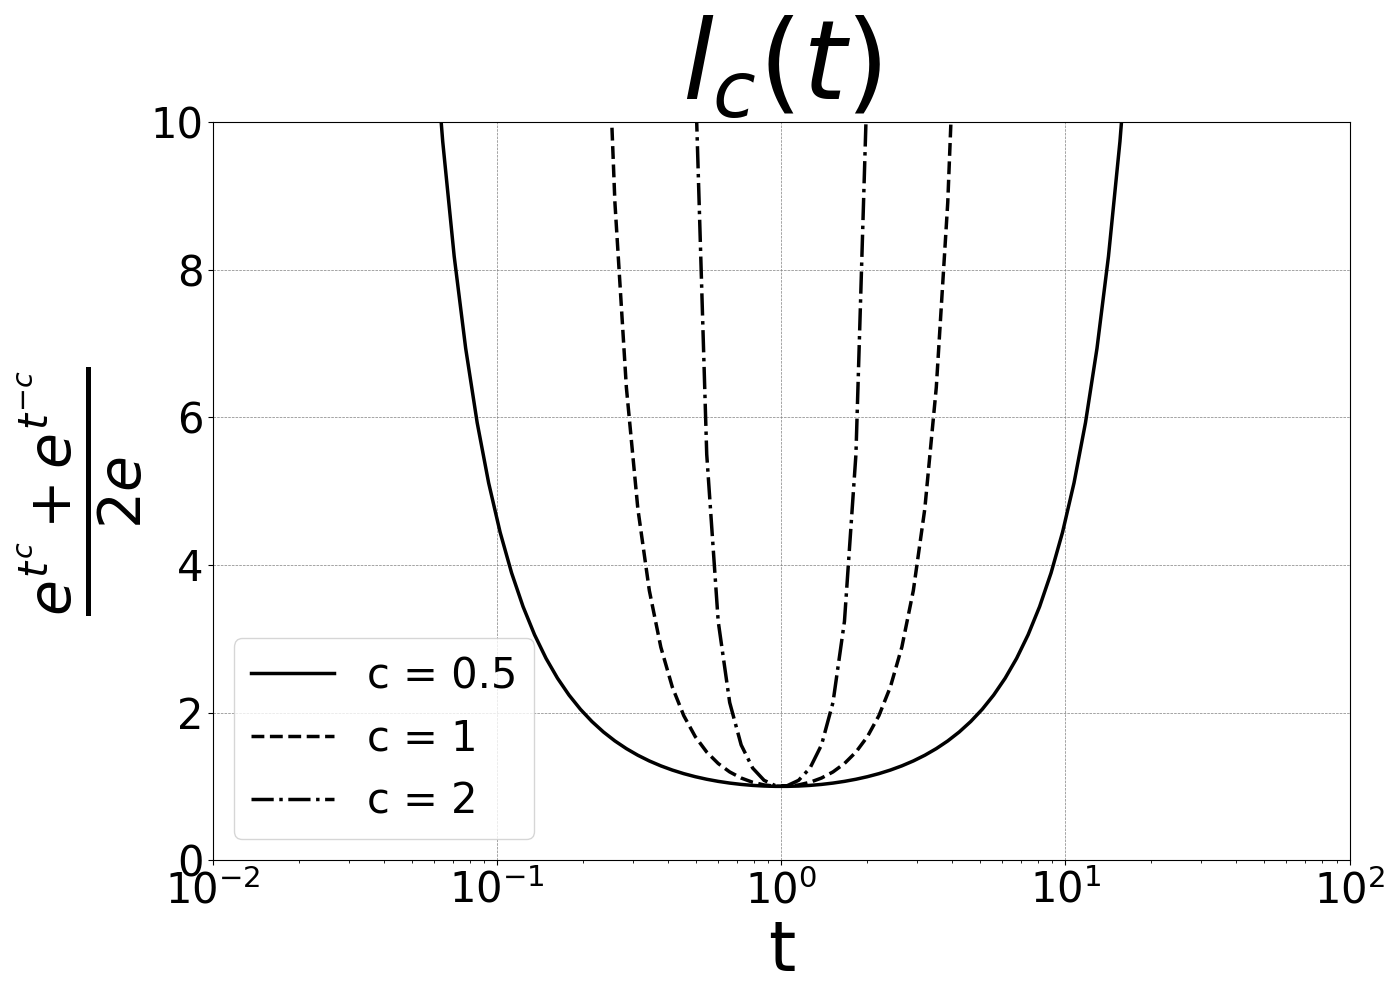
\includegraphics[width = .32\textwidth]{../figures/Figure_1a_bw.png}}
\subcaptionbox{Normalized length vs. unnormalized length\label{fig:normalized_length}}
{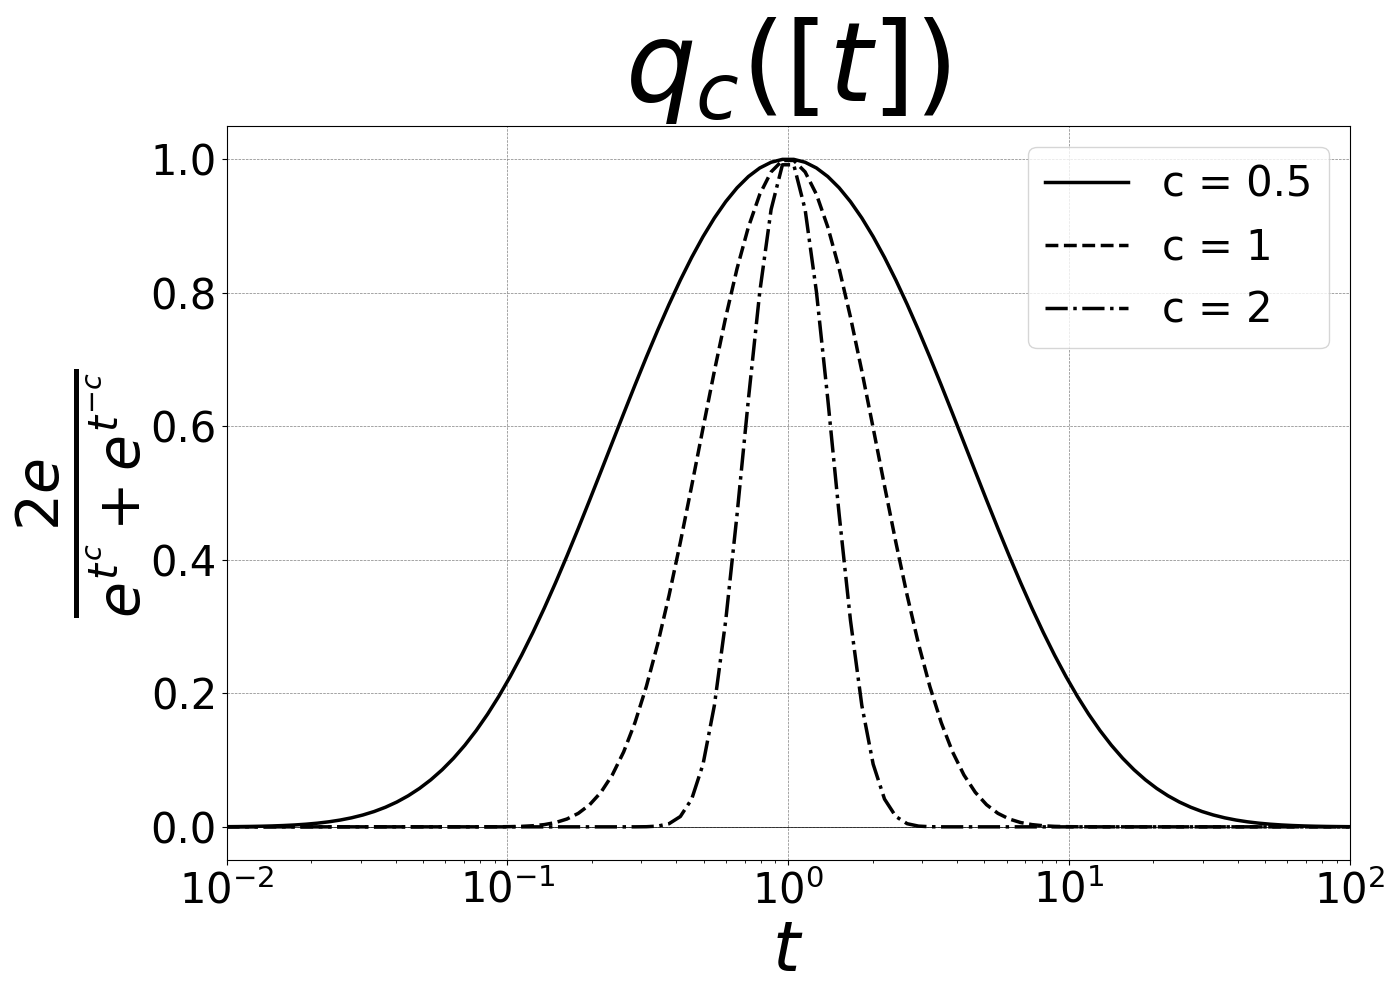
\includegraphics[width = .32\textwidth]{../figures/Figure_1b_bw.png}}
\subcaptionbox{Basis pursuit loss\label{fig:bp_loss}}
{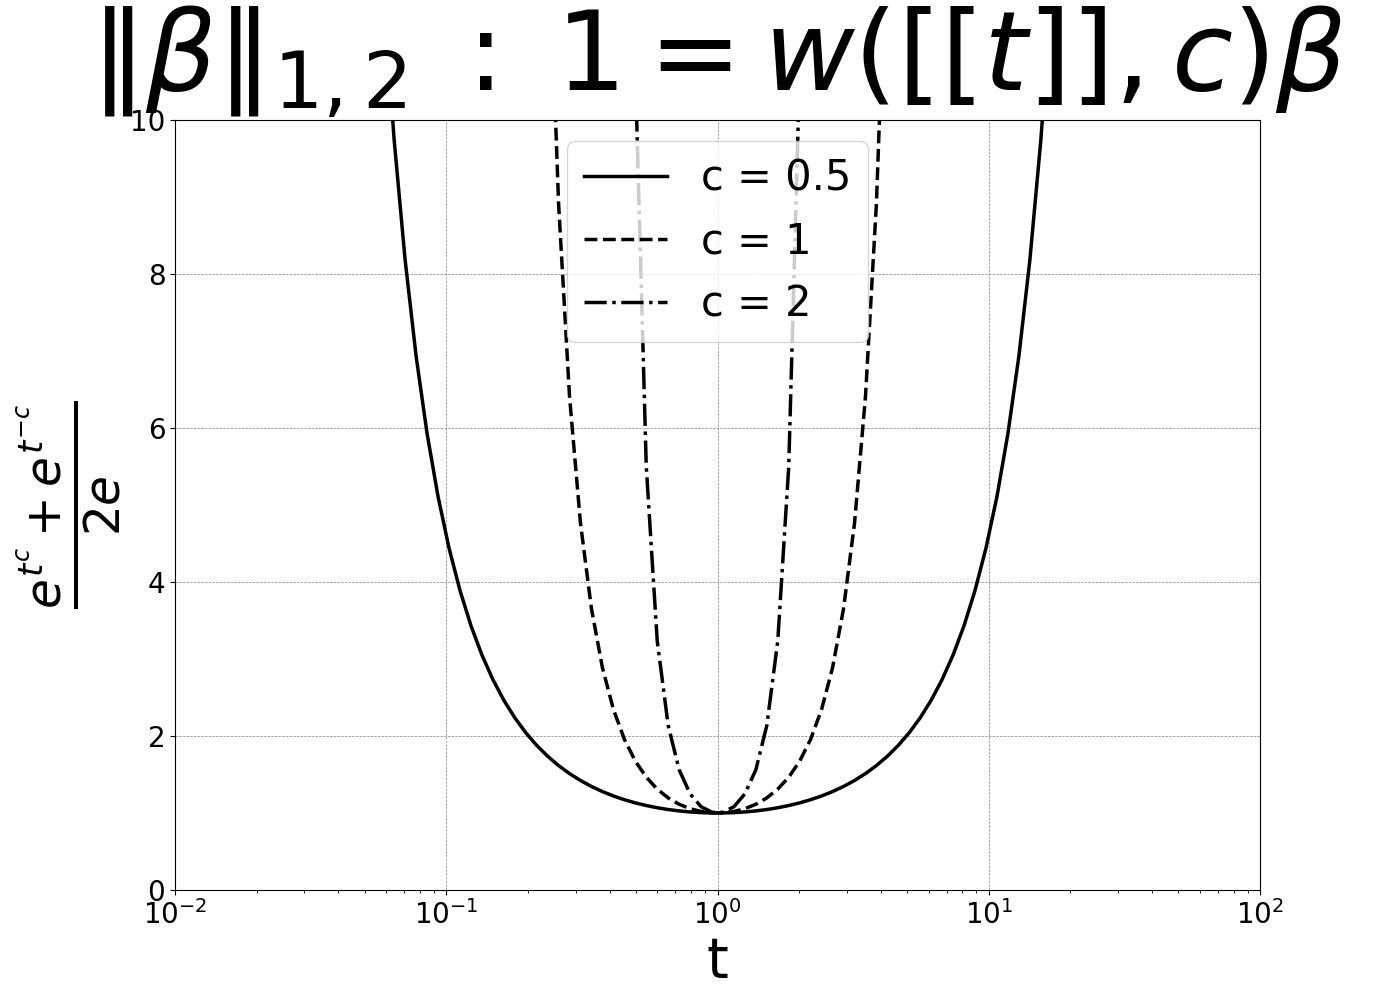
\includegraphics[width = .32\textwidth]{../figures/Figure_1c_bw.png}}

\caption{\ref{fig:data} Raw data $X$ represented as column-vectors.
 \ref{fig:selection} An isometric subset - the identification of which is our objective.
 \ref{fig:normalization} The vectors after normalization so that vectors of length $1$ maintain longest length.
 \ref{fig:gt_loss} Our ground truth loss function for different values of $c$ in the one-dimensional case $D = 1$
 \ref{fig:normalized_length} Normalized length used to rescale Figure \ref{fig:data} to get vectors in Figure \ref{fig:normalization}.
 \ref{fig:bp_loss} Basis pursuit loss. 
This loss is equivalent to that shown in Figure \ref{fig:gt_loss} in the one-dimensional case.
\label{fig:losses}
}
\end{figure}

\section{Method}

We apply the group lasso paradigm used to select independent dictionary elements in \citet{Koelle2022-ju, Koelle2024-no} to the more specific problem of selecting pointwise isometries from a dictionary.
We first define a ground truth objective computable via brute and greedy algorithms that is uniquely minimized by orthonormal matrices.
We then define the combination of normalization and multitask basis pursuit that approximates this ground truth loss function.
We finally give a brute post-processing method for ensuring that the solution is $D$ sparse, and provide a theoretical result that the two stage approach will always result in recovery of an isometric solution from the dictionary, should one exist.

\subsection{Ground truth}
\label{sec:ground_truth}

We'd like a ground truth objective to be minimized uniquely by orthonormal matrices, invariant under rotation, and depend on all changes in the matrix.
Deformation \citep{Kohli2021-lr} and nuclear norm \citep{Boyd2004-ql} use only a subset of the differential's information and are not uniquely minimized at unitarity, respectively.
We therefore introduce an alternative ground truth objective that satisfies the above desiderata and has convenient connections to isometry pursuit.

This ground truth objective is
\begin{align}
l_{c}: \mathbb R^{D \times P} &\to \mathbb R^{+} \\
X &\mapsto \sum_{d = 1}^D g(\sigma_d( X), c)
\end{align}
where $\sigma_d ( X)$ is the $d$-th singular value of $ X$ and
\begin{align}
g: \mathbb R^+ \times \mathbb R^+ &\to \mathbb R^+ \\
t,c &\mapsto \frac{e^{t^c} + e^{t^{-c}}}{2e}.
\end{align}
By Proposition \ref{prop:orthonormal_spectrum}, we can see that $\ell_c$ is uniquely maximized by orthonormal matrices.
Moreover, $g$ is convex, and $\ell_c( X^{-1}) = \ell_c( X)$ when $X$ is invertible.
Figure \ref{fig:gt_loss} gives a graph of $l_c$ when $D=1$.



% compares it with that produced by basis pursuit after normalization as in Section \ref{sec:normalization}.
% NOTE (Sam): Do we need proofs of maximized by orthonormal matrices and convex?
% Can we prove this is a norm?

Our ground truth objective is therefore the best subset selection problem
\begin{align}
\label{prog:ground_truth}
\arg \min_{ S \in \binom{[P]}{d}} l_c ( X_{. S}).
\end{align}
Regardless of the convexity of $l_c$, brute combinatorial search over $[P]$ is inherently non-convex.
This motivates our alternative formulation.

\subsection{Normalization}
\label{sec:normalization}

Since basis pursuit methods tend to select longer vectors, selection of orthonormal submatrices requires normalization such that both long and short candidate basis vectors are penalized in the subsequent regression.
We introduce the following definition.

\begin{definition}[Symmetric normalization]
A function $q: \mathbb R^D \to \mathbb R^+ $ is a symmetric normalization if 
\begin{align}
\arg \max_{v \in \mathbb R^D} \ q (v) &=\{ v : \|v\|_2 = 1 \} \\
q(v) &= q(\frac{v}{\|v\|_2^2}) \\
q(v_1) &= q(v_2) \; \forall \; v_1, v_2 \in \mathbb R^D : \|v_1\|_2 = \|v_2\|_2.
\end{align} \label{def:symmetric_normalization}
\end{definition}

We use such functions to normalize column-vector length in such a way that vectors of length $1$ prior to normalization have longest length after normalization and vectors are shrunk proportionately to their deviation from $1$. 
That is, we normalize vectors by 
\begin{align}
n: \mathbb R^D  &\to \mathbb R^D \\
v &\mapsto {q(v) }v
\end{align}
and matrices by
\begin{align}
w: \mathbb R^{D \times P}  &\to \mathbb R^D \\
 X_{.p} &\mapsto n( X_{.p}) \; \forall \; p \in [P].
\end{align}

Given $c > 0$, we choose $q$ as follows.
\begin{align}
q_c: \mathbb R^D  &\to \mathbb R^+ \\
v  &\mapsto \frac{e^{\|v\|_2^c} + e^{\|v\|_2^{-c}}}{2e}.
\label{eq:normalization}
\end{align}

Besides satisfying the conditions in Definition \ref{def:symmetric_normalization}, this normalization has some additional nice properties.
First, $q$ is convex.
Second, it grows asymptotically log-linearly.
Third, while $\exp(-|\log t|) = \exp(-\max (t, 1/t))$ is a seemingly natural choice for normalization, it is non smooth, and the LogSumExp \citep{Boyd2004-ql} replacement of $\max (t, 1/t)$ with $ \log (\exp (t ) + \exp(1/t))$ simplifies to \ref{eq:normalization} upon exponentiation.
Finally, the parameter $c$ grants control over the width of the basin, which may be useful for avoiding numerical issues arising close to $0$ and $\infty$.
We plot this normalization function in Figure \ref{fig:normalized_length} and its effect on our example data in Figure \ref{fig:normalization}.



\subsection{Isometry pursuit}

Isometry pursuit is the application of multitask basis pursuit to the normalized design matrix $w(X, c)$ to identify submatrices of $ X$ that are as orthonormal as possible.
Define the multitask basis pursuit penalty 
\begin{align}
\label{eq:bp}
\| \cdot \|_{1,2}: \mathbb R^{P \times D} &\to \mathbb R^+ \\ 
\beta &\mapsto  \sum_{p=1}^P  \|\beta_{p.}\|_2.
\end{align}
Given a matrix $Y \in \mathbb R^{D \times D}$, the multitask basis pursuit solutions are
\begin{align}
\label{prog:multitask_basis_pursuit}
\widehat {\mathcal {\beta}}_{MBP} (X, Y)  := \arg \min_{\beta \in \mathbb R^{P \times D}} \| \beta \|_{1,2} \; : \;Y =  X \beta.
\end{align}

Note that multitask basis pursuit solution is not unique under more relaxed conditions than for standard basis pursuit.
Recall that, given a design matrix $X$, there exists a response variable $y$ such that the lasso admits a non-unique solution if and only if the rowspan of the design matrix $X$ contains a sufficient codimension edge of the $p$ dimensional hypercube \citep{Schneider2022-hi}.
This condition generalizes the previously introduced general position condition - that affinely independent columns of the design matrix guarantee non-uniqueness.
However, for Isometry Pursuit, non-unique solutions may occur even when this condition is satisfied.
A simple example -
$X =
\begin{bmatrix}
1 & 0 & \frac{\sqrt{2}}{2} & \frac{\sqrt{2}}{2}  \\
0 & 1 & \frac{\sqrt{2}}{2} & \frac{-\sqrt{2}}{2}  
\end{bmatrix}$
results from the rotation invariance Proposition \ref{prop:unitary_selection}, but more subtle examples exist.
We therefore define
\begin{align}
\widehat \beta^{l_2}_{MLP} (X,Y) = \arg \min \|\beta\|_F : \beta \in \mathcal \beta_{MBP} (X, Y) .
\end{align}
By the strong convexity of the $l_2$ norm, $\widehat \beta^{l_2}_{MLP} (X,Y)$ is well defined.

This implicit regularization assumption is reasonable.
% Mishkin2023-yt is broken
For example, in \citet{Tibshirani2012-vw} the implicit selection of the minimum $l_2$ norm solution among the lasso solutions was proven for the Least Angle Regression Selection (LARS) algorithm for solving the lasso, while \citet{Mishkin2022-yf}  assumes that the group lasso solution is in fact min-norm prior to subsequent theoretical analyses.
Empirically, the Splitting Conic Solver type method (which is itself a variant of the Alternating Direction Method of Multilpliers) \citep{O-Donoghue2013-wf} stably estimates the min-norm solution when initialized at $0$, but besides a brief exploration in Section \ref{sec:deep_dive} we leave theoretical and experimental proof of this feature of the feature our optimization approach for future work, and instead make the ability of our optimizer to obtain the min-norm solution an assumption of our eventual proposition.

Isometry pursuit is then given by
\begin{align}
\label{prog:isometry_pursuit}
\widehat \beta_c ( X) := \widehat \beta_{MBP}^{l_2} ( w(X,c), I_D )
\end{align}
where $I_D$ is the $D$ dimensional identity matrix and recovered functions are the indices of the dictionary elements with non-zero coefficients.
That is, they are given by $S(\beta)$ where
\begin{align}
S: \mathbb{R}^{P \times D} &\to \binom{[P]}{D} \\
\beta &\mapsto \left\{ p \in [P] :  \|\beta_{p.}\| > 0 \right\}.
\end{align}
\begin{algorithm}[H]
\caption{\isometrypursuit(Matrix ${X} \in \mathbb{R}^{D \times P}$, scaling constant $c$)}
\begin{algorithmic}[1]
\STATE {Normalize} $X_c = w({X},c)$
\STATE {Optimize} $\widehat \beta = \widehat \beta_{MBP}^{l_2} (X_c, I_D)$
\STATE {\bf Output} $\widehat{S} = S (\widehat \beta)$
\end{algorithmic}
\end{algorithm}

\subsection{Theory}

The intuition behind our application of multitask basis pursuit is that submatrices consisting of vectors which are closer to 1 in length and more orthogonal will have smaller loss.
A key theoretical assertion is that \isometrypursuit~ is invariant to choice of basis for $ X$.
\begin{proposition}
\label{prop:basis_pursuit_selection_invariance}
Let $U \in \mathbb R^{D \times D}$ be orthonormal.
Then $S(\widehat \beta  (U  X)) = S(\widehat \beta ( X))$.
\end{proposition}
This proposition establishes the basis-independence of Isometry Pursuit and that we may replace $I_D$ in the constraint by any orthonormal $D \times D$ matrix.
It is also essential for showing the following main theoretical result.

When a rank $D$ orthonormal column-submatrix $X_{.S}$ exists, the output of Program \ref{prog:isometry_pursuit} will contain $S$.
\begin{proposition}
Let $X \in \mathbb R^{D \times P}$ have a rank $D$ orthonormal column submatrix $X_{.S}$.
Then $S \subseteq \widehat \beta_c ( X)$.
\label{prop:unitary_selection}
\end{proposition}

Proofs of these propositions are given in Section \ref{sec:proofs}, with corresponding experimental results in Section \ref{sec:experiments}.
The proof mostly relies on the KKT conditions \citep{Hastie2015-qa} being used to verify that an isometric subset yields a corresponding basis pursuit solution for an appropriate normalized matrix.
This is a formalization of our intuition that longer and more orthogonal vectors will minimize loss.
We then apply a simple argument to show that the $l_2$ minimizing solution is the least sparse solution, which means that it contains the isometry solution, should it exist.

\subsection{Two-stage isometry pursuit}

Proposition \ref{prop:unitary_selection} suggests the following algorithm, which first uses the convex \isometrypursuit~ algorithm to prune the $P$ candidate features and then applies brute search upon the reduced feature set.
Similar two-stage approaches are standard in the Lasso literature \cite{Hesterberg2008-iy, Koelle2022-ju}, and Proposition \ref{prop:unitary_selection} puts them on relatively strong footing in our application, since this approach is guaranteed to select an isometric submatrix should one exist.
This method forms our practical isometry estimator, the core advantage of which over purely brute search is a substantially reduced feature set.

\begin{algorithm}[H]
\caption{\tsip(Matrix ${X} \in \mathbb{R}^{D \times P}$, scaling constant $c$)}
\begin{algorithmic}[1]
\STATE $\widehat{S}_{IP} = \text{\isometrypursuit}( X, c)$
\STATE $\widehat{S} = \text {\brute}({X}_{.\widehat{S}_{IP}}, l_c)$
\STATE {\bf Output} $\widehat{S}$
\end{algorithmic}
\end{algorithm}

